\section{Grammar as network of finite automata}

Let's $G$ be an EBNF with each nonterminal having a single rule $A \rightarrow \alpha$, where $\alpha$ is a regular expression comprising terminals and nonterminals.
The regular expression $\alpha$ defines a regular language, and thus, there exists a finite state automaton $M_A$ that recognizes $\alpha$.

In the grammar $G$, a transition labeled with nonterminal $B$ is interpreted as a call to the automaton $M_B$.
If $B=A$, the call is considered recursive.

\begin{definition}[\textit{Machines}]
    The finite state automata associated with the nonterminals of $G$ are referred to as machines. 
\end{definition}
\begin{definition}[\textit{Automaton}]
    The pushdown machine that analyzes the language generated by $G$, denoted as $L(G)$, is termed automaton. 
\end{definition}
\begin{definition}[\textit{Network}]
    The set of all the machines of $G$ is called network.
\end{definition}
The components utilized to define a network include:
\begin{enumerate}
    \item The alphabet of the terminal symbols: $\Sigma$
    \item The alphabet of the nonterminal symbols: $V=\{S,A,B,\dots\}$.
    \item The grammar rules: $S \rightarrow \sigma$, $A \rightarrow \alpha$, $B \rightarrow \beta$, etc. 
    \item The regular languages over $\Sigma \cup V$ defined by $\sigma, \alpha, \beta$, etc.: $R_S,R_A,R_B$, etc. 
    \item The deterministic finite machine recognizing $R_S,R_A,R_B$, etc.: $M_S,M_A,M_B$, etc. 
    \item The machine network: $\mathcal{M}=\{M_S,M_A,M_B,\dots\}$
\end{enumerate}

It is crucial to consider the terminal language defined by a general machine $M_A$, even when commencing from a state that may not be the initial one.
For any state $q_A$, regardless of its initial status, we express it as:
\[L(M_A,q_A)=\{y \in \Sigma^{*}|\exists\eta\in R(M_A,q) \land \overset{*}{\underset{G}{\implies}} y\}\]
The above formula encompasses a string $\eta$ composed of terminals and non-terminals, accepted by the machine $M_A$ when initiated in state $q$. 
The derivations originating from $\eta$ generate all terminal strings within the language $L(q)$. 
Notably, this implies:
\[L(M_A,0_A)=L(0_A) = L_A(G)\]
Similarly, for the axiom:
\[L(M_S,0_S)=L(0_S)=L_S(G) = L(\mathcal{M})\]

An additional constraint must be imposed: the initial state $0_A$ of machine $A$ should not be re-entered after the computation's initiation.
This condition is easily satisfied; at worst, the machine requires a new initial state.
Automata satisfying this constraint are referred to as normalized.
\begin{example}
    Let's examine the grammar governing arithmetic expressions:
    \[\begin{cases}
        E \rightarrow [+|-]T((+|-)T)^{*} \\
        T \rightarrow F((\times|/)F)^{*} \\
        F \rightarrow a | '('E')'
    \end{cases}\]   
    The associated network is illustrated below:
    \begin{figure}[H]
        \centering
        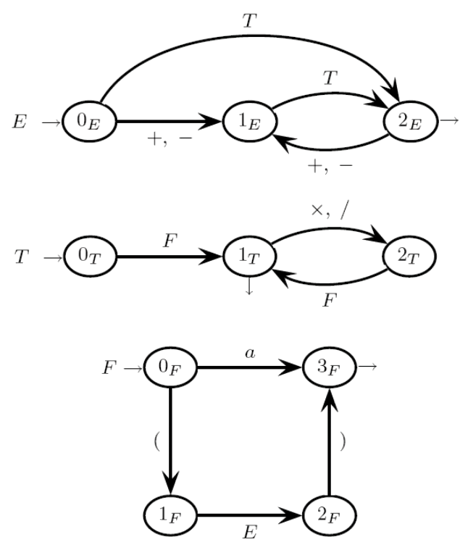
\includegraphics[width=0.4\linewidth]{images/net.png}
    \end{figure}
    It is noteworthy that the machine $T$ has been normalized.
\end{example}

\paragraph*{Procedures for networks}
These networks can be translated into programs that utilize recursion. 
The code of the program mirrors the machine transitions. 
When the finite automaton has a branching state, determining the direction to take requires examining all symbols on the arcs leaving the state, including the final transitions of the machine.
\begin{example}
    The machine network from the previous example can be converted into three code procedures. 
    The procedure for the grammar $E$ is as follows:
    \begin{algorithmic}[1]
        \State call $T$
        \While {$cc=+$}
            \State $cc:=next$
            \State call $T$
        \EndWhile
        \If {$cc \in \{(\dashv\}$}
            \State \Return
        \Else 
            \State error
        \EndIf
    \end{algorithmic}
    The procedure for the grammar $T$ is presented below:
    \begin{algorithmic}[1]
        \State call $F$
        \While {$cc=\times$}
            \State $cc:=next$
            \State call $F$
        \EndWhile
        \If {$cc \in \{(+\dashv\}$}
            \State \Return
        \Else 
            \State error
        \EndIf
    \end{algorithmic}
    The procedure for the grammar $F$ is outlined as follows:
    \begin{algorithmic}[1]
        \If {$cc=a$}
            \State $cc:=next$
        \ElsIf {$cc=($}
            \State $cc:=next$
            \State call $E$
            \If {$cc=)$}
                \State $cc:=next$
                \If {$cc \in \{) \times \dashv\}$}
                    \State \Return
                \Else 
                    \State error
                \EndIf
            \Else 
                \State error
            \EndIf
        \Else 
            \State error
        \EndIf
    \end{algorithmic}
\end{example}